\ProvidesFile{chapters/ch-Event_Selection.tex}

\chapter{DATASETS, EVENT SELECTION, AND \ensuremath{\mathrm{t\bar{t}}} KINEMATIC RECONSTRUCTION}
\label{Datasets_Event_Selection_Kinematic_Reconstruction}

\begin{cabstract}
test test test test test test test
\end{cabstract}

The signal process for this measurement is the production of top quark pairs followed by top quark decays $t\to W^+ b$ and $\bar{t}\to W^- \bar{b}$, and subsequent leptonic $W$ boson decays into final state muons $W\to \mu\nu$ and electrons $W\to e\nu$, both ``prompt'' and ``via tau,'' i.e. via the decay of the W boson into a tau $W\to \tau\nu$ and its subsequent leptonic decay into a final state electron $\tau\to e\nu$ or muon $\tau\to \mu\nu$.
The analysis has been carried out using the CMS EDM and official software framework for event generation, simulation, and reconstruction, following recommendations for ultra-legacy Run II analyses by the Physics Performance and Datasets (PPD) and the Physics Data And Monte Carlo Validation (PdmV) CMS groups.

\section{Datasets}

\subsection{Recorded Datasets}
These measurements are performed using \lumivalueSixPreVFP $\pm$ \lumierrSixPreVFP~\cite{bib:lumipas16}, \lumivalueSixPostVFP $\pm$ \lumierrSixPostVFP~\cite{bib:lumipas16}, \lumivalueSeven $\pm$ \lumierrSeven~\cite{bib:lumipas17}, and \lumivalueEight $\pm$ \lumierrEight~\cite{bib:lumipas18} (Total: \lumivalueRuniiUL $\pm$ \lumierrRuniiUL) of data collected with the CMS experiment at the LHC with \beamenergy, during 2016, 2017, and 2018 respectively.
Only the runs and luminosity sections that had good functioning of every CMS sub-detector were selected for analysis.
The measurements are performed using ultra legacy CMS data sets, which are comprehensively documented, designed to be useful for a wide range of studies, preserved for long-term access, and include high-level physics objects such as reconstructed leptons, jets, and missing transverse energy.
The 2016 data set is separated into ``preVFP'' and ``postVFP'', partitioning the year into the periods before and after heavily ionizing particle mitigation (HIPM) was implemented, while no such separation for the 2017 or 2018 data sets exist.

\subsection{Simulated Datasets}
MC simulations (described in section~\ref{Monte_Carlo_Event_Simulation}) are used to estimate signal and background contributions. 
The dileptonic \ttbar signal sample is produced using the \Powheg\ event generator with NLO ME calculations. 
PS and hadronization of the \ttbar signal sample is performed using \Pythia. 
The matrix-element jets are matched to parton showers using the \Powheg\ method. 
The MC simulations assume that $m_t = \SI{172.5}{\GeV}$, and the PDFs are described using NNPDF3.1.

The major sources of background contributions are semi-leptonic \ttbar, fully hadronic \ttbar, dileptonic decays of single top quarks in association with a $W$ boson ($tW$ and $\bar{t}W$), \ttbar in association with $W/Z$ bosons, \zjets, \wjets, and $WW$, $WZ$, $ZZ$ diboson processes. 
A summary of the MC simulations for signal and background processes is shown in table~\ref{simulated_Datasets}, including the ME generator, PS algorithm, and cross-section used for luminosity scaling.

\begin{table}[htb]
\caption{A summary of the MC simulations for signal and background processes including the ME generator, PS algorithm, and cross-section used for luminosity scaling.
  }
\vspace*{6pt}
 \begin{center}
   \begin{adjustbox}{scale=0.75,center}
    \begin{tabular}
      {lccr} \hline Process & ME (Matching) & PS & $\sigma$ [pb]\\
      \hline
      { \ttbar (Dileptonic)} & \Powheg & \Pythia &  $\xsecTTBARdilept$ \\
      { \ttbar (Semi-Leptonic)} & \Powheg & \Pythia &  $\xsecTTBARljets$ \\
      { \ttbar (Hadronic)} & \Powheg & \Pythia &  $\xsecTTBARhadronic$ \\
      { $\ttbar+W$ (Leptonic $W$)} & \MGaMCatNLOOnly+\MadSpin & \Pythia &  $\xsecTTWJETSlnu$ \\
      { $\ttbar+W$ (Hadronic $W$)} & \MGaMCatNLOOnly+\MadSpin & \Pythia &  $\xsecTTWJETSqq$ \\
      { $\ttbar+Z$ (Leptonic $Z$)} & \MG & \Pythia &  $\xsecTTZllnunu$ \\
      { $\ttbar+Z$ (Hadronic $Z$)} & \MG & \Pythia &  $\xsecTTZqq$ \\
      { $t+W$ (Dileptonic)} & \Powheg & \Pythia &  $\xsecSINGLETOPtw$ \\
      { $\bar{t}+W$ (Dileptonic)} & \Powheg & \Pythia &  $\xsecSINGLETOPtw$ \\
      { $W+\text{Jets}$} & \MG & \Pythia &  $\xsecWlnu$ \\
      { $Z/\gamma^*+\text{Jets} \quad (\SI{10}{\GeV} < m_{\ell\bar{\ell}} < \SI{50}{\GeV})$} & \MG & \Pythia &  $\xsecDYTenFifty$ \\
      { $Z/\gamma^*+\text{Jets} \quad (m_{\ell\bar{\ell}} > \SI{50}{\GeV})$} & \MG & \Pythia &  $0.5 \times \xsecDYFiftyInf$ \\
      { $Z/\gamma^*+\text{Jets} \quad (m_{\ell\bar{\ell}} > \SI{50}{\GeV})$} & \MGaMCatNLO & \Pythia &  $0.5 \times \xsecDYFiftyInf$ \\
      { $WW$} & \Pythia & \Pythia &  $\xsecWW$ \\
      { $WZ$} & \Pythia & \Pythia &  $\xsecWZ$ \\
      { $ZZ$} & \Pythia & \Pythia &  $\xsecZZ$ \\
      \hline
      \end{tabular}
   \end{adjustbox}
  \label{simulated_Datasets}     
 \end{center}
\end{table}

\section{Particle-Flow Reconstruction and Event Selection}
The CMS detector consists of several sub-detector layers that exploit the different properties of particles to identify them and measure their energy-momenta and trajectories.
For reconstructing particle objects from their interaction with the detector, the CMS experiment has developed a holistic particle-flow (PF) reconstruction algorithm that combines the measurements from all relevant sub-detector layers~\cite{Sirunyan:2270046}.
The algorithm links the charged-particle tracks measured in the inner silicon tracker with the energy deposits in the calorimeters and the muon tracks measured in the outer muon tracking system.
As there are trade-offs between reconstruction efficiency and misidentification rate, the criteria for classifying reconstructed objects are determined by dedicated CMS Physics Object Groups (POG) which perform expert analyses to optimize the efficiency and purity of object identification.

The main particles that are directly detected by CMS are muons, electrons, photons, charged hadrons (e.g. protons, pions, kaons), and neutral hadrons (e.g. neutrons).
An illustration of the signatures left behind by these particles in the various sub-detectors is shown in figure~\ref{CMS_Layers}.
\begin{figure}[htb]
  \begin{center}
    \begin{tabular}{c}
        \includegraphics[width=0.99\textwidth]{fig_LHC_CMS/CMS_Layers.png}
    \end{tabular}
    \caption{Muons, electrons, photons, charged hadrons, and neutral hadrons are directly detected by CMS and are identified by the signatures they leave behind in the various sub-detectors~\cite{Sirunyan:2270046}.
            }
    \label{CMS_Layers}
  \end{center}
\end{figure}
The PF algorithm identification and reconstruction sequence first identifies and reconstructs muon candidates, then electron and photon candidates, and finally charged and neutral hadron candidates.
After each step, tracks and clusters of reconstructed objects are removed from further consideration for subsequent steps.

For the measurements presented in this dissertation, the reconstruction of the different objects is performed using the PF algorithm and the object identification criteria follow the recommendations for ultra-legacy Run II analyses by the CMS Top Physics Analysis Group (Top PAG).
The \ttbar dilepton final state is characterized by the presence of at least two high-\pT isolated leptons with opposite electric charge, large MET (\ETmiss), and two jets created from the hadronization of $b$-quarks.

\subsection{Triggers}
To maximize the trigger efficiency, dilepton data streams and single-lepton streams are both used for this measurement.
In order to ensure no double-counting of events, events passing the dilepton triggers are vetoed when processing the single lepton data streams.
Approximately 10\% of dilepton events that failed to pass the dilepton trigger requirements are recovered by including the single lepton data streams.
The trigger efficiency is measured in data as a function of the lepton \pT and used to correct the MC simulations.

\subsection{Track and Vertex Reconstruction, Primary Vertex Requirements, and Pileup Corrections}
Every $\SI{25}{\ns}$, an average bunch crossing results in 1000 or more particles from 20 or more $pp$ collisions~\cite{Chatrchyan:1129810}.
Track reconstruction is the determination of final state particle trajectories using the ionization trails left behind in the tracker sub-detector layers and is crucial for the identification and momenta measurement of charged particles.
The situation where multiple $pp$ collisions (vertices) occur within the same bunch crossing is referred to as PU, and vertexing is the determination of vertices from the intersection of trajectories.
The primary vertex (PV) of an event is the vertex corresponding to the hard-scattering interaction in the collision and is identified as the vertex with the highest sum of squared transverse momenta of its associated tracks.
Vertexing is also important for the identification of secondary vertices (SV), i.e. vertices separated from the beamline by $\gtrsim \SI{1}{\mm}$, which are usually attributed to the decay of short-lived heavy flavor mesons.

In the PF algorithm, iterative Kalman filtering (KF) is used to reconstruct the tracks and vertices of charged particles~\cite{Sirunyan:2270046}.
KF assumes that the residuals between the predicted and measured trajectories are Gaussian distributions.
The algorithm is seeded with tracks generated from two hits in consecutive layers in the pixel detector.
The KF fits the expected trajectory of the particles based on measured charge and momentum, accounts for multiple scattering and energy loss of particles in the detector material, and updates the track parameters based on measurements in each detector layer.
A visualization of the reconstructed tracks and identified vertices for an event with high PU recorded by the CMS detector in 2016 is shown in figure~\ref{Pileup}.
\begin{figure}[htb]
  \begin{center}
    \begin{tabular}{c}
        \includegraphics[width=0.6\textwidth]{fig_Event_Reconstruction/Pileup.png}
    \end{tabular}
    \caption{A visualization of the reconstructed tracks and identified vertices for an event with high PU recorded by the CMS detector in 2016~\cite{Collaboration:2231915}.
            }
    \label{Pileup}
  \end{center}
\end{figure}

For the measurements presented in this dissertation, the PV of an event is required to be associated with at least four tracks and be in the vicinity of the nominal interaction point with $\vert r \vert < \SI{2}{\cm}$ and $\vert z \vert < \SI{24}{\cm}$. 
Charged-hadron subtraction (CHS) is used to remove charged PU contributions and the L1FastJet algorithm is applied to subtract the remaining neutral contributions~\cite{bib:JME18001}.
The number of PU events in MC simulations is typically based on an estimate of the expected number of interactions per bunch crossing and PU re-weighting is performed using the instantaneous luminosity per bunch crossing in data, and the total $pp$ inelastic cross section of $\SI{69.2}{\milli \b}$, to correct the PU distribution of the MC simulation.

\subsection{Muons}
\label{PF_Reconstruction_Muons}
Muons leave tracks in the silicon tracker, their trajectories are curved due to the presence of the magnetic field of the solenoid, and they penetrate through the calorimeters and solenoid to leave ionization trails in the chambers of the muon system.
As is implied by its name, the CMS experiment was designed to detect muons with high reconstruction efficiency and low misidentification rate.
Muons that are reconstructed independently in both the inner tracking detector and the outer muon system are referred to as global muons.
A global fit of the muon momentum using both sub-detectors has momentum resolution of $1-3\%$ for low momentum muons ($\SI{20}{\GeV} < \pT < \SI{200}{\GeV}$), depending on $\eta$, and $5\%$ for high momentum muons (\sim$\SI{1}{\TeV}$)~\cite{Chatrchyan:1129810}.
If hadron shower remnants ``punch-through'' the HCAL and solenoid into the outer muon system, they may be misreconstructed as muons, but additional criteria can be used to balance the efficiency and purity of muon identification.

For the measurements presented in this dissertation, PF muon candidates are required to have a transverse momentum $\pT > \SI{20}{\GeV}$ and a pseudorapidity restricted to the coverage of the inner tracker $\vert \eta \vert < 2.4$.
They are also required to be reconstructed as global muons and fulfill tight selection criteria chosen to ensure high purity, provide good \pT measurements, and suppress punch-through fake-muons and muons produced from hadron decays.
To remove leptons overlapping with jets, PF muon candidates are required to fulfill the isolation condition $I^{PF}_{Rel}< 0.15$.
Corrections are also applied that scale the raw energy measurements and smear the muon resolutions to match the accuracy and precision of reconstructed muons in MC simulation to those in recorded data.
Identification and isolation efficiency corrections for muons are also applied and are measured as a function of \pT and $\eta$ using a ``tag-and-probe'' method with an orthogonal dataset.

\subsection{Electrons}
\label{PF_Reconstruction_Electrons}
Electrons leave ionization trails in the silicon tracker, their trajectories are curved due to the presence of the magnetic field of the solenoid, and their energy is deposited in the ECAL.
Electron tracks are seeded from the ECAL clusters and extrapolated back to the inner silicon tracker.
Gaussian Sum Filtering (GSF), which assumes that the residuals between the predicted and measured trajectories are sums of multiple Gaussian distributions, is used to reconstruct electrons.
Due to the total radiation length of the inner silicon tracker, the probability that an electron emits a bremsstrahlung photon by interacting with tracker material is about $85\%$~\cite{Sirunyan:2270046}.
Thus the ECAL clusters from the electron and the bremsstrahlung photons in a window around the electron direction are grouped into a ``supercluster.''
For non-isolated electrons, such as those produced in jets, the superclustering can result in large inefficiencies, so the ECAL seeding criteria are restricted by isolation requirements.

For the measurements presented in this dissertation, PF electron candidates are required to have transverse momentum $\pT > \SI{20}{\GeV}$ and a pseudorapidity restricted to the coverage of the inner tracker $\vert \eta \vert < 2.4$.
The gap between the barrel and endcap region of the ECAL ($1.4442 < \vert \eta_\mathrm{sc} \vert < 1.5660$) is excluded, where $\eta_\mathrm{sc}$ is the pseudorapidity of the ECAL supercluster.
To ensure high purity, electron selection uses tight identification and isolation criteria.
The electron isolation considers photons, neutral hadrons, and charged hadrons as identified by the PF algorithm in a $\eta$-$\phi$ space cone of $\Delta R < 0.3$ around the electron.
Corrections are also applied that scale the raw energy measurements and smear the electron resolutions to match the accuracy and precision of reconstructed electrons in MC simulation to those in recorded data.
Identification and reconstruction efficiency corrections for electrons are also applied and are measured as a function of \pT and $\eta$ using a ``tag-and-probe'' method with an orthogonal dataset.

\subsection{Lepton Pair}
Events with a dilepton system consisting of exactly two oppositely-charged leptons passing the electron and muon object selection criteria are accepted for further consideration.
If more than two leptons are reconstructed in the event, then the event is vetoed.
The leading selected lepton is required to have $\pT > \SI{25}{\GeV}$.
The event is then unambiguously classified as \ee, \emu, or \mumu depending on the type of the selected lepton pair.
The invariant mass of the selected lepton pair is required to be larger than $\SI{20}{\GeV}$ to suppress background events from decays of heavy-flavor resonances and Drell-Yan processes.
Moreover, in the \ee and \mumu decay channels, events are rejected if the dilepton invariant mass is within the vicinity of the $Z$ boson mass $\SI{76}{\GeV} < m_{\ell\bar{\ell}} < \SI{106}{\GeV}$, where background from $Z$ boson production is dominant.

\subsection{Jets}
\label{PF_Reconstruction_Jets}
Quarks and gluons produced in $pp$ collisions hadronize into collimated showers of particles called jets.
Jets primarily consist of hadrons, but also can contain photons and leptons when hadrons in the jet radiate or decay before reaching the detector.
Charged hadrons leave tracks in the silicon tracker, have curved trajectories due to the presence of the magnetic field of the solenoid, deposit some energy in the ECAL, and exhaust their energy in the HCAL, while neutral hadrons do not leave tracks in the silicon tracker and exhaust their energy in the HCAL.
The granularity of the inner silicon tracker is sufficiently fine to provide separation of individual particle trajectories within jets, and energy clusters are deposited in the calorimeters from the particles in the shower.

The anti-$k_T$ jet clustering algorithm groups reconstructed PF objects into jets by merging the pair of particles with the smallest distance, calculating new distances between the merged object and the remaining particles, and repeating this process until all particles have been merged into jet objects~\cite{Matteo_Cacciari_2008}.
For anti-$k_T$ jet clustering, the distance $d_{ij}$ between two particles $i$ and $j$ is defined as:
\begin{linenomath*}
\begin{align}
d_{ij} = min(\sfrac{1}{p_{T,i}^2}, \sfrac{1}{p_{T,j}^2}) \times \sfrac{{\Delta R_{ij}}^2}{R^2}
\end{align}
\end{linenomath*}
where $\Delta R$ is the angular separation between objects, defined in equation~\ref{DeltaR}, and $R$ is the radius parameter that determines the size of individual jets.
The PF algorithm reduces the amount of energy that is mistakenly assigned to a jet due to PU by removing clusters attributed to tracks originating at PU vertices.
Due to complications such as assumptions about particle separation in the clustering algorithm, energy loss in the detector material, detector noise, PU, detector granularity, the association of neutral hadrons with interaction vertices, and the stochastic nature of particle showers in the HCAL, reconstructed jet energies and trajectories are typically associated with large systematic uncertainties.

For the measurements presented in this dissertation, jets are clustered from reconstructed PF candidates using the anti-$k_T$ clustering algorithm with radius parameter $R = 0.4$ (AK4).
Events are required to have at least two jets with transverse momentum $\pT > \SI{30}{\GeV}$ and within the coverage of the inner tracker $\vert \eta \vert < 2.4$. 
Identification criteria is applied to efficiently identify jets (efficiency \sim $98\% - 99\%$) while rejecting jets with significant lepton fractions (purity \sim $98\%$).
To exclude jets overlapping with selected leptons used in the analysis, a cleaning of leptons from jets is applied if $\Delta R(jet,lepton)<0.4$.
Events with jets in regions of the calorimeter that produced anomalously high or low jet rates are vetoed in MC and recorded data.

Jet energy corrections (JEC) are applied that adjust the jet energy scale (JES) to match the accuracy of reconstructed jet energies in MC simulation to those in recorded data.
To reduce the contribution coming from PU, the CHS algorithm removes charged particles and the L1FastJet algorithm removes the remaining neutral contributions from PU vertices before clustering jets~\cite{bib:JME18001}.
L2L3 MC-truth corrections are applied to both data and MC simulation to correct for the variation of detector resolution as a function of jet $\eta$ and \pT.
Any remaining discrepancies in the accuracy of jet energy measurements due to detector response and other effects are eliminated with the application of L2L3Residual corrections.
Jet energy resolution (JER) corrections are applied by smearing the jets in MC simulation to match the precision of jets in recorded data.

\subsection{Missing Transverse Energy}
For collisions at the LHC, there is no net momentum or force in the transverse direction, so \pT is conserved and sums to zero for both incoming protons and outgoing particles after the collision.
This property is useful for inferring the production of particles invisible to the detector, i.e. neutrinos, from the missing transverse energy (MET):
\begin{linenomath*}
\begin{align}
\vec{E}_T^{miss}=-\sum_{i} \vec{p}_{T,i}
\end{align}
\end{linenomath*}
the negative vector sum of the transverse momenta for all PF reconstructed particles in an event, illustrated in figure~\ref{met_schematic}.
\begin{figure}[htb]
  \begin{center}
    \begin{tabular}{c}
        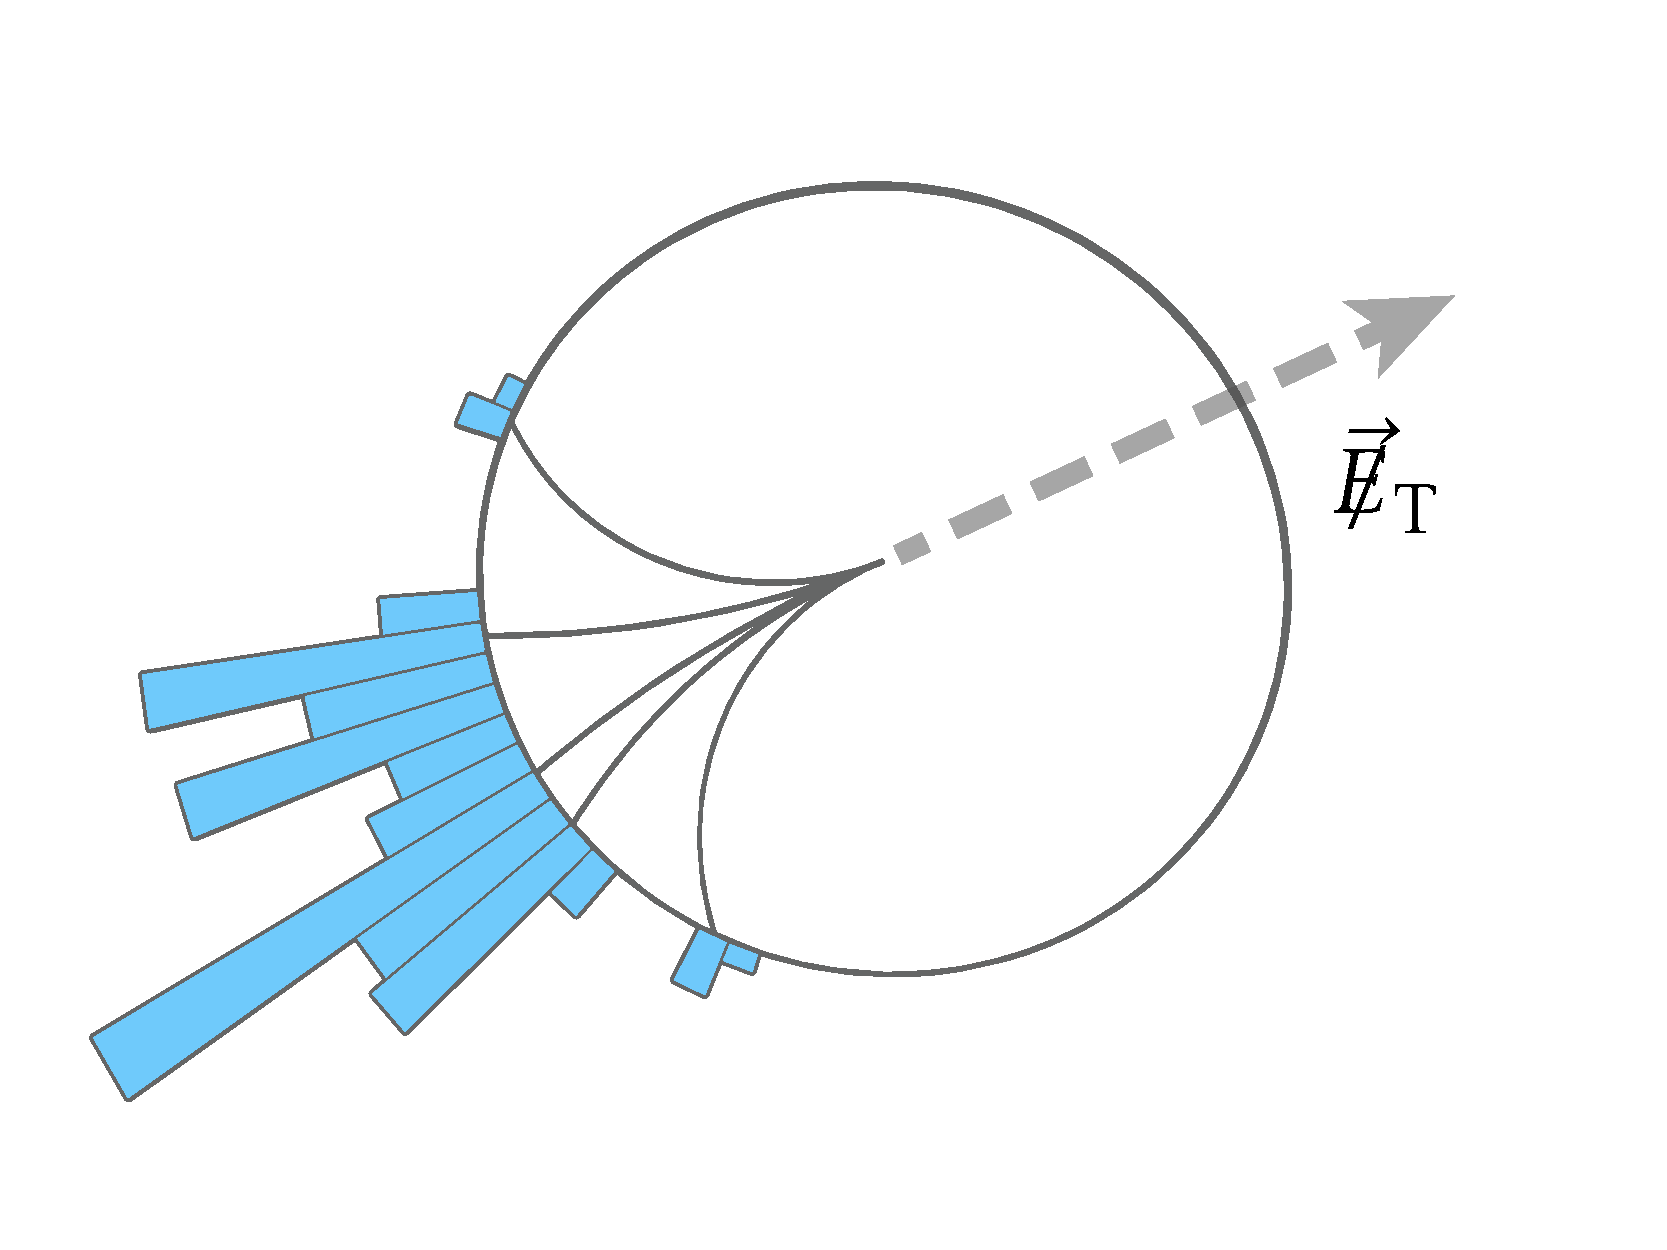
\includegraphics[width=0.5\textwidth]{fig_Event_Reconstruction/met_schematic.pdf}.
    \end{tabular}
    \caption{Schematic diagram for \MET, the negative vector sum of the transverse momenta for all reconstructed particles in an event~\cite{METSchematicDiagram}.
            }
    \label{met_schematic}
  \end{center}
\end{figure}

For the measurements presented in this dissertation, the calculation of the \ETmiss is based on PF objects, where pileup-per-particle-identification (PUPPI)~\cite{bib:PUPPI} is used for PU mitigation.
PUPPI is an alternative to the PF CHS algorithm which gives weights to particles based on the probability that they come from PU or the PV.
The JEC (JES and JER) and lepton energy scale corrections are propagated to the \ETmiss.
Events in the \ee and \mumu channels are required to have $\ETmiss > \SI{40}{\GeV}$, but no requirement on \ETmiss is applied in the \emu channel.

\subsection{Tagging of b-Jets}
Selected events are required to have at least one jet tagged as having originated from a $b$-quark.
In this analysis, the DeepJet $b$-tagging algorithm~\cite{bib:Bols_2020}, which uses approximately 650 input variables, divided into four categories (global variables, charged PF candidate features, neutral PF candidate features, and SV features associated with the jet) as inputs for a deep neural network, is used to tag all reconstructed jets in the event.
A DeepJet medium working point is used with light ($l$)-jet mistag efficiency of \sim$1\%$ (see figure~\ref{bTagging}).
\begin{figure}[htb]
  \begin{center}
    \begin{tabular}{cc}
        \includegraphics[width=0.40\textwidth]{fig_Event_Selection/Secondary_Vertex.png}
        \includegraphics[width=0.40\textwidth]{fig_Event_Selection/DeepJet.png}
    \end{tabular}
    \caption{Illustration of a heavy-flavor jet with a SV from the decay of a $b$ or $c$ hadron resulting in charged-particle tracks (including possibly a soft lepton) that are displaced with respect to the PV, and hence with a large impact parameter (IP) value (Right)~\cite{app122010574}.
    Misidentification probability for $c$ and $l$-jets versus $b$ jet identification efficiency for DeepJet and DeepCSV $b$ tagging algorithms applied to jets in \ttbar events~\cite{app122010574}.
            }
    \label{bTagging}
  \end{center}
\end{figure}

\subsection{Event Selection Control Plots}
\begin{figure}[htb]
    \begin{center}
        \begin{tabular}{cc}
            \includegraphics[width=0.40\textwidth]{fig_fullRun2UL/controlplots/combined/DIMFull.pdf}
            \includegraphics[width=0.40\textwidth]{fig_fullRun2UL/controlplots/combined/HypjetMulti_diLep.pdf}
        \end{tabular}
        \caption{\footnotesize Dilepton invariant mass and jet multiplicity distributions for combined 2016preVFP, 2016postVFP, 2017, 2018 eras and combined \ee, \emu, \mumu channels after selection of two isolated leptons passing the trigger requirements and $m_{\ell\bar{\ell}} > \SI{20}{\GeV}$.
        For the jet multiplicity distribution, events in the \ee and \mumu channels with $\SI{76}{\GeV} < m_{\ell\bar{\ell}} < \SI{106}{\GeV}$ have also been rejected.
        The simulated samples are re-weighted to an integrated luminosity of \lumivalueRuniiUL.
        Trigger efficiency and lepton selection scale factors discussed in section~\ref{Experimental_Systematics} are applied.
        No \zjets\ scaling has been applied yet.
        Statistical uncertainties are shown as error bars on the data points, and total systematic uncertainties are indicated by the hatched uncertainty band.
        }
    \end{center}
\end{figure}

\begin{figure}[htb]
    \begin{center}
        \begin{tabular}{cc}
            \includegraphics[width=0.40\textwidth]{fig_fullRun2UL/controlplots/combined/MET_preMETcut.pdf}
            \includegraphics[width=0.40\textwidth]{fig_fullRun2UL/controlplots/combined/HypBjetMulti_noBTag.pdf}
        \end{tabular}
        \caption{\footnotesize \ETmiss and $b$-tagged jet multiplicity distribution for combined 2016preVFP, 2016postVFP, 2017, 2018 eras and combined \ee, \emu, \mumu channels after selection of two isolated leptons passing the trigger requirements, $m_{\ell\bar{\ell}} > \SI{20}{\GeV}$, $N_{jets} \geq 2$, and rejecting events in the \ee and \mumu channels with $\SI{76}{\GeV} < m_{\ell\bar{\ell}} < \SI{106}{\GeV}$.
        For the $b$-tagged jet multiplicity distribution, events in the \ee and \mumu channels with $\ETmiss < \SI{40}{\GeV}$ have also been rejected.
        The simulated samples are re-weighted to an integrated luminosity of \lumivalueRuniiUL.
        Trigger efficiency, lepton selection, and $b$-tagging efficiency scale factors discussed in section~\ref{Experimental_Systematics} are applied.
        The \zjets\ contributions in MC have been scaled to better describe the number of events observed in recorded data, as discussed in section~\ref{Zjets_Background_Determination}.
        Statistical uncertainties are shown as error bars on the data points, and total systematic uncertainties are indicated by the hatched uncertainty band.        
        }
    \end{center}
\end{figure}

\begin{figure}[htb]
    \begin{center}
        \begin{tabular}{cc}
            \includegraphics[width=0.40\textwidth]{fig_fullRun2UL/controlplots/combined/HypLeptonpT.pdf}
            \includegraphics[width=0.40\textwidth]{fig_fullRun2UL/controlplots/combined/HypLeptonEta.pdf} \\
            \includegraphics[width=0.40\textwidth]{fig_fullRun2UL/controlplots/combined/HypAntiLeptonpT.pdf}
            \includegraphics[width=0.40\textwidth]{fig_fullRun2UL/controlplots/combined/HypAntiLeptonEta.pdf}
        \end{tabular}
        \caption{\footnotesize \pT and $\eta$ distributions for selected leptons and anti-leptons for combined 2016preVFP, 2016postVFP, 2017, 2018 eras and combined \ee, \emu, \mumu channels after all object and event selection criteria have been applied.
        The simulated samples are re-weighted to an integrated luminosity of \lumivalueRuniiUL.
        Trigger efficiency, lepton selection, $b$-tagging efficiency, and kinematic reconstruction efficiency scale factors discussed in section~\ref{Experimental_Systematics} are applied.
        The \zjets\ contributions in MC have been scaled to better describe the number of events observed in recorded data, as discussed in section~\ref{Zjets_Background_Determination}.
        Statistical uncertainties are shown as error bars on the data points, and total systematic uncertainties are indicated by the hatched uncertainty band.
        }
        \label{lepton_control}
    \end{center}
\end{figure}

\clearpage
\section{\ensuremath{\mathrm{t\bar{t}}} Kinematic Reconstruction}

\subsection{Full \ensuremath{\mathrm{t\bar{t}}} Kinematic Reconstruction}
To fully pass event selection, an event is also required to have at least one solution to the \ttbar kinematic reconstruction.
The top quark and anti-quark are fully reconstructed using an analytical method~\cite{Sonnenschein:2006ud}, in which eight kinematic constraints are applied to determine the unknown four-momenta of the undetected neutrinos.
The constraint equations are constructed from the four-momenta of the objects passing event selection: two leptons, two jets, and the missing transverse energy. 
The two neutrinos are assumed to be massless:
\begin{linenomath*}
\begin{align}
m_{\nu}^2 &= E_{\nu}^2 - \sum_{i = x, y, z} p_{\nu_i}^2 = 0 \\
m_{\bar{\nu}}^2 &= E_{\bar{\nu}}^2 - \sum_{i = x, y, z} p_{\bar{\nu}_i}^2 = 0
\end{align}
\end{linenomath*}
The missing transverse energy is assumed to be entirely from the transverse momenta of the two neutrinos:
\begin{linenomath*}
\begin{align}
E_{x}^{\text{miss}}=p_{\nu_x}+p_{\bar{\nu}_x} \\
E_{y}^{\text{miss}}=p_{\nu_y}+p_{\bar{\nu}_y}
\end{align}
\end{linenomath*}
The lepton (anti-lepton) and the anti-neutrino (neutrino) are assumed to have an invariant mass equal to the W boson mass of $m_{W^\pm} = \SI{80.4}{\GeV}$:
\begin{linenomath*}
\begin{align}
m_{W^{+}}^2 &=\left(E_{\bar{\ell}}+E_\nu\right)^2- \sum_{i = x, y, z} \left(p_{\bar{\ell}_i}+p_{\nu_i}\right)^2  \\
m_{W^{-}}^2 &=\left(E_{\ell}+E_{\bar{\nu}}\right)^2- \sum_{i = x, y, z} \left(p_{\ell_i}+p_{\bar{\nu}_i}\right)^2
\end{align}
\end{linenomath*}
Finally, the reconstructed top quark and anti-quark are assumed to have an invariant mass of $m_{t} = m_{\bar{t}} = \SI{172.5}{\GeV}$:
\begin{linenomath*}
\begin{align}
m_t^2 &= \left(E_{\bar{\ell}}+E_\nu+E_b\right)^2- \sum_{i = x, y, z} \left(p_{\bar{\ell}_i}+p_{\nu_i}+p_{b_i}\right)^2 \\
m_{\bar{t}}^2 &= \left(E_{\ell}+E_{\bar{\nu}}+E_{\bar{b}}\right)^2 - \sum_{i = x, y, z} \left(p_{\ell_i}+p_{\bar{\nu}_i}+p_{\bar{b}_i}\right)^2 
\end{align}
\end{linenomath*}
The constraint equations can be simplified to a single $4^{\text{th}}$ order polynomial equation for one of the neutrino four-momenta components, which can be solved analytically with up to a four-fold ambiguity to obtain the neutrino and top quark four-momenta.
If an event may contain more than two $b$-jet candidates, then each pair of jet--lepton assignments are tried.
Jets $b$-tagged by the DeepJet algorithm are tried first, and only if no solution is found are the untagged jets considered.
The solution which yields the minimum invariant mass of the \ttbar system has been shown~\cite{PhysRevD.73.112006} to provide, in most cases, the solution with correct jet--lepton assignments and is the method used in this measurement to resolve the ambiguities arising from having multiple solutions.

Due to fluctuations in the measured jet momenta and missing transverse energy, the simplified constraint equation is not always solvable.
To enhance reconstruction efficiency, each event is reconstructed 100 times with different random smearings of jet and lepton energies and directions within their resolutions.
The resolutions are determined using the signal MC simulation after event selection by comparing the reconstructed jet and lepton energies and directions to the true $b$-quark and lepton values.
The jet and lepton energies are smeared by randomly sampling a distribution of the ratio of the true energy divided by the reconstructed energy (the ratio distributions are shown in figure~\ref{fig:energyFactor}).
The directions are smeared randomly about the reconstructed direction with magnitude sampled from a Gaussian distribution with the resolution taken from the average of the angular difference between the reconstructed and true directions (the distributions from which the average resolutions were obtained are shown in figure~\ref{fig:angleFactor}).
The $W$ boson masses used in the constraints are also smeared randomly about their central values using the width of their relativistic Breit-Wigner mass distribution (shown in figure~\ref{fig:inputDists}).

\begin{figure}[htb]
    \begin{center}
        \includegraphics[width=0.35\textwidth]{fig_fullRun2UL/SmearingPlots/ULcomp_KinReco_fE_jet_step7.pdf}
        \includegraphics[width=0.35\textwidth]{fig_fullRun2UL/SmearingPlots/ULcomp_KinReco_fE_lep_step7.pdf}
        \caption{\small Distributions of the true energy divided by the reconstructed energy used for the energy smearing in the \ttbar full kinematic reconstruction. 
        The factors are shown for the b quarks (left) and the leptons (right).}
    \label{fig:energyFactor}
    \end{center}
\end{figure}

\begin{figure}[htb]
    \begin{center}
        \includegraphics[width=0.35\textwidth]{fig_fullRun2UL/SmearingPlots/ULcomp_KinReco_d_angle_jet_step7.pdf}
        \includegraphics[width=0.35\textwidth]{fig_fullRun2UL/SmearingPlots/ULcomp_KinReco_d_angle_lep_step7.pdf}
        \caption{\small Distributions of the angle between the true direction and the reconstructed direction for jets (left) and leptons (right).}
       \label{fig:angleFactor}
    \end{center}
\end{figure}

\begin{figure}[htb]
    \begin{center}
        \includegraphics[width=0.35\textwidth]{fig_fullRun2UL/SmearingPlots/ULcomp_KinReco_W_mass_step0.pdf}
        \includegraphics[width=0.35\textwidth]{fig_fullRun2UL/SmearingPlots/ULcomp_KinReco_mbl_true_step0.pdf}
        \caption{\small Distributions of the true W boson mass (left) and invariant mass distribution of reconstructed leptons and $b$-jets (right).}
       \label{fig:inputDists}
    \end{center}
\end{figure}

Likelihood weights for each smeared solution are calculated from the invariant mass of reconstructed leptons and $b$-jets relative to the true invariant mass distributions.
The true lepton-$b$-jet invariant mass distribution used to calculate solution likelihood weights is shown in figure~\ref{fig:inputDists}.
For each smearing, the jet--lepton assignment that yields the maximum weight is chosen.
A weighted average of all smeared solutions provides the final solution to the top quark three-momentum:
\begin{align}
%\langle \vec{p}_{t} \rangle = \frac{1}{w_s} \sum_{i=1}^{100} w_i \cdot \vec{p}_{t,\,i} \quad \mbox{with} \quad w_s = \sum_{i=1}^{100} w_{i}
\langle \vec{p}_{t} \rangle = \frac{1}{w(m_{\ell b})_{\Sigma}} \sum_i^{100} w(m_{\ell b})_i \cdot \vec{p}_{t_i}
\end{align}
where $w(m_{\ell b})_i$ and $\vec{p}_{{t}_i}$ denote the weight and reconstructed top quark three-momentum obtained for the $i$-th smearing of the event.
Smearings without any solutions are given null weights.
The top quark energy is calculated from its three-momentum and the top quark mass constraint $m_{t} = \SI{172.5}{\GeV}$.
The final solution for the top anti-quark four-momentum is determined in an analogous procedure.

\clearpage
\subsection{Kinematic Reconstruction Control Plots}
Kinematic reconstruction control distributions for solutions to the kinematic reconstruction for combined 2016preVFP, 2016postVFP, 2017, 2018 eras and combined \ee, \emu, \mumu channels after all object and event selection criteria have been applied are shown in figure~\ref{bjet_control} for $b$-jets, figure~\ref{leptonbjet_control} for lepton and $b$-jet invariant mass, figure~\ref{top_control} for top quarks, and figure~\ref{ttbar_control} for the \ttbar\ system.
The \pT spectra of top quarks and anti-quarks in \ttbar\ data are known to be softer than modeled by MC simulations.
Modeling systematics associated with this deficiency are discussed in section~\ref{Model_Systematics} and it is also evident in the \pT distributions of downstream top quark decay products such as those for leptons (figure~\ref{lepton_control}) and $b$-jets (figure~\ref{bjet_control}).


\begin{figure}[htb]
    \begin{center}
        \begin{tabular}{cc}
            \includegraphics[width=0.40\textwidth]{fig_fullRun2UL/controlplots/combined/HypBJetpT.pdf}
            \includegraphics[width=0.40\textwidth]{fig_fullRun2UL/controlplots/combined/HypBJetEta.pdf} \\
            \includegraphics[width=0.40\textwidth]{fig_fullRun2UL/controlplots/combined/HypAntiBJetpT.pdf}
            \includegraphics[width=0.40\textwidth]{fig_fullRun2UL/controlplots/combined/HypAntiBJetEta.pdf} 
        \end{tabular}
        \caption{\footnotesize \pT and $\eta$ distributions for $b$-jet and anti-$b$-jet solutions to the kinematic reconstruction for combined 2016preVFP, 2016postVFP, 2017, 2018 eras and combined \ee, \emu, \mumu channels after all object and event selection criteria have been applied.
        The simulated samples are re-weighted to an integrated luminosity of \lumivalueRuniiUL.
        Trigger efficiency, lepton selection, $b$-tagging efficiency, and kinematic reconstruction efficiency scale factors discussed in section~\ref{Experimental_Systematics} are applied.
        The \zjets\ contributions in MC have been scaled to better describe the number of events observed in recorded data, as discussed in section~\ref{Zjets_Background_Determination}.
        Statistical uncertainties are shown as error bars on the data points, and total systematic uncertainties are indicated by the hatched uncertainty band.
        }
        \label{bjet_control}
    \end{center}
\end{figure}

\begin{figure}[htb]
    \begin{center}
        \begin{tabular}{cc}
            \includegraphics[width=0.40\textwidth]{fig_fullRun2UL/controlplots/combined/HypAntiLeptonBjetMass.pdf}
            \includegraphics[width=0.40\textwidth]{fig_fullRun2UL/controlplots/combined/HypLeptonBjetMass.pdf}
        \end{tabular}
        \caption{\footnotesize Left (Right): Kinematic reconstruction solutions for anti-lepton and $b$-jet (lepton and anti-$b$-jet) invariant mass distributions for combined 2016preVFP, 2016postVFP, 2017, 2018 eras and combined \ee, \emu, \mumu channels after all object and event selection criteria have been applied.
        The simulated samples are re-weighted to an integrated luminosity of \lumivalueRuniiUL.
        Trigger efficiency, lepton selection, $b$-tagging efficiency, and kinematic reconstruction efficiency scale factors discussed in section~\ref{Experimental_Systematics} are applied.
        The \zjets\ contributions in MC have been scaled to better describe the number of events observed in recorded data, as discussed in section~\ref{Zjets_Background_Determination}.
        Statistical uncertainties are shown as error bars on the data points, and total systematic uncertainties are indicated by the hatched uncertainty band.
        }
        \label{leptonbjet_control}
    \end{center}
\end{figure}

\begin{figure}[htb]
    \begin{center}
        \begin{tabular}{cc}
            \includegraphics[width=0.40\textwidth]{fig_fullRun2UL/controlplots/combined/HypToppT.pdf}
            \includegraphics[width=0.40\textwidth]{fig_fullRun2UL/controlplots/combined/HypTopRapidity.pdf} \\
            \includegraphics[width=0.40\textwidth]{fig_fullRun2UL/controlplots/combined/HypAntiToppT.pdf}
            \includegraphics[width=0.40\textwidth]{fig_fullRun2UL/controlplots/combined/HypAntiTopRapidity.pdf} 
        \end{tabular}
        \caption{\footnotesize \pT and $y$ distributions for the top quark and anti-top quark solutions to the kinematic reconstruction for combined 2016preVFP, 2016postVFP, 2017, 2018 eras and combined \ee, \emu, \mumu channels after all object and event selection criteria have been applied.
        The simulated samples are re-weighted to an integrated luminosity of \lumivalueRuniiUL.
        Trigger efficiency, lepton selection, $b$-tagging efficiency, and kinematic reconstruction efficiency scale factors discussed in section~\ref{Experimental_Systematics} are applied.
        The \zjets\ contributions in MC have been scaled to better describe the number of events observed in recorded data, as discussed in section~\ref{Zjets_Background_Determination}.
        Statistical uncertainties are shown as error bars on the data points, and total systematic uncertainties are indicated by the hatched uncertainty band.
        The \pT spectra of top quark and anti-quarks in \ttbar\ data are known to be softer than modeled by MC simulations, and modeling systematics associated with this deficiency are discussed in section~\ref{Model_Systematics}.
        }
        \label{top_control}
    \end{center}
\end{figure}

\begin{figure}[htb]
    \begin{center}
        \begin{tabular}{ccc}
            \includegraphics[width=0.40\textwidth]{fig_fullRun2UL/controlplots/combined/HypTTBarMass.pdf} \\
            \includegraphics[width=0.40\textwidth]{fig_fullRun2UL/controlplots/combined/HypTTBarpT.pdf} 
            \includegraphics[width=0.40\textwidth]{fig_fullRun2UL/controlplots/combined/HypTTBarRapidity.pdf} \\
        \end{tabular}
        \caption{\footnotesize \pT, $y$, and invariant mass distributions for \ttbar solutions to the kinematic reconstruction for combined 2016preVFP, 2016postVFP, 2017, 2018 eras and combined \ee, \emu, \mumu channels after all object and event selection criteria have been applied.
        The simulated samples are re-weighted to an integrated luminosity of \lumivalueRuniiUL.
        Trigger efficiency, lepton selection, $b$-tagging efficiency, and kinematic reconstruction efficiency scale factors discussed in section~\ref{Experimental_Systematics} are applied.
        The \zjets\ contributions in MC have been scaled to better describe the number of events observed in recorded data, as discussed in section~\ref{Zjets_Background_Determination}.
        Statistical uncertainties are shown as error bars on the data points, and total systematic uncertainties are indicated by the hatched uncertainty band.
        }
        \label{ttbar_control}
    \end{center}
\end{figure}

\clearpage
\subsection{Comparison of \ensuremath{\mathrm{t\bar{t}}} Reconstruction for Prompt and Via \ensuremath{\mathrm{\tau}} Dilepton Events}
The assumption that the dilepton decay is prompt and there are only two neutrinos in the final state is not true when the dilepton decay is via intermediate $\tau$ leptons; such decays can have four or six neutrinos in the final state.
The top quark and \ttbar reconstructed kinematic variables at detector-level (rec) are presented versus the true variables at generator level (gen), and additionally, the resolutions are presented as the difference between the true and reconstructed variables in bins of the true variables. 
Figures~\ref{fig:kinrec:resolution-mtt} through~\ref{fig:kinrec:resolution-yt} show the resolutions of \mtt, \ytt, \pttt, \yt, and \ptt\ for both prompt and via tau reconstructed \ttbar dilepton events. 
The means and standard deviation parameters (sigmas) from Gaussian fits to the kinematic variable resolutions are also included and reflect the bias and resolution of the algorithm, including degradation attributed to wrong jet--lepton assignments. 
From the sigmas of the fits, we conclude that the kinematic variable resolutions of \ttbar dilepton events via $\tau$ are \sim$5\% - 15\%$ degraded relative to prompt events, but are sufficiently comparable to be included as signal in this measurement.

\begin{figure}
  \begin{center}
    \includegraphics[width=0.35\textwidth]{fig_fullRun2UL/KinRecoResolutions/ttbar_mass_genreco_prompt.pdf}
    \includegraphics[width=0.35\textwidth]{fig_fullRun2UL/KinRecoResolutions/ttbar_mass_genreco_viatau.pdf}\\
    \includegraphics[width=0.35\textwidth]{fig_fullRun2UL/KinRecoResolutions/ttbar_mass_residual_prompt.pdf}
    \includegraphics[width=0.35\textwidth]{fig_fullRun2UL/KinRecoResolutions/ttbar_mass_residual_viatau.pdf}\\
    \includegraphics[width=0.35\textwidth]{fig_fullRun2UL/KinRecoResolutions/ttbar_mass_multiresidual_prompt.pdf}
    \includegraphics[width=0.35\textwidth]{fig_fullRun2UL/KinRecoResolutions/ttbar_mass_multiresidual_viatau.pdf}\\
    \caption{\small Top: True and reconstructed \mtt\ obtained for prompt (left) and via tau (right) \ttbar dilepton events.
    Middle: The difference between true and reconstructed \mtt\ in bins of true \mtt\ (fitted with a Gaussian function for illustration).
    Bottom: The differential mean and sigma from Gaussian fits, with respect to true \mtt, of the difference between true and reconstructed \mtt\ obtained for prompt and via tau \ttbar dilepton events.
    The simulated samples are normalized to an integrated luminosity of \lumivalueRuniiUL.}
    \label{fig:kinrec:resolution-mtt}
 \end{center}
\end{figure}

\begin{figure}
  \begin{center}
    \includegraphics[width=0.35\textwidth]{fig_fullRun2UL/KinRecoResolutions/ttbar_pT_genreco_prompt.pdf}
    \includegraphics[width=0.35\textwidth]{fig_fullRun2UL/KinRecoResolutions/ttbar_pT_genreco_viatau.pdf}\\
    \includegraphics[width=0.35\textwidth]{fig_fullRun2UL/KinRecoResolutions/ttbar_pT_residual_prompt.pdf}
    \includegraphics[width=0.35\textwidth]{fig_fullRun2UL/KinRecoResolutions/ttbar_pT_residual_viatau.pdf}\\
    \includegraphics[width=0.35\textwidth]{fig_fullRun2UL/KinRecoResolutions/ttbar_pT_multiresidual_prompt.pdf}
    \includegraphics[width=0.35\textwidth]{fig_fullRun2UL/KinRecoResolutions/ttbar_pT_multiresidual_viatau.pdf}\\
    \caption{\small Top: True and reconstructed \pttt\ obtained for prompt (left) and via tau (right) \ttbar dilepton events.
    Middle: The difference between true and reconstructed \pttt\ in bins of true \pttt\ (fitted with a Gaussian function for illustration).
    Bottom: The differential mean and sigma from Gaussian fits, with respect to true \pttt, of the difference between true and reconstructed \pttt\ obtained for prompt and via tau \ttbar dilepton events.
    The simulated samples are normalized to an integrated luminosity of \lumivalueRuniiUL.}
    \label{fig:kinrec:resolution-pttt}
 \end{center}
\end{figure}

\begin{figure}
  \begin{center}
    \includegraphics[width=0.35\textwidth]{fig_fullRun2UL/KinRecoResolutions/ttbar_rapidity_genreco_prompt.pdf}
    \includegraphics[width=0.35\textwidth]{fig_fullRun2UL/KinRecoResolutions/ttbar_rapidity_genreco_viatau.pdf}\\
    \includegraphics[width=0.35\textwidth]{fig_fullRun2UL/KinRecoResolutions/ttbar_rapidity_residual_prompt.pdf}
    \includegraphics[width=0.35\textwidth]{fig_fullRun2UL/KinRecoResolutions/ttbar_rapidity_residual_viatau.pdf}\\
    \includegraphics[width=0.35\textwidth]{fig_fullRun2UL/KinRecoResolutions/ttbar_rapidity_multiresidual_prompt.pdf}
    \includegraphics[width=0.35\textwidth]{fig_fullRun2UL/KinRecoResolutions/ttbar_rapidity_multiresidual_viatau.pdf}\\
    \caption{\small Top: True and reconstructed \ytt\ obtained for prompt (left) and via tau (right) \ttbar dilepton events.
    Middle: The difference between true and reconstructed \ytt\ in bins of true \ytt\ (fitted with a Gaussian function for illustration).
    Bottom: The differential mean and sigma from Gaussian fits, with respect to true \ytt, of the difference between true and reconstructed \ytt\ obtained for prompt and via tau \ttbar dilepton events.
    The simulated samples are normalized to an integrated luminosity of \lumivalueRuniiUL.}
    \label{fig:kinrec:resolution-ytt}
 \end{center}
\end{figure}

\begin{figure}
  \begin{center}
    \includegraphics[width=0.35\textwidth]{fig_fullRun2UL/KinRecoResolutions/top_pT_genreco_prompt.pdf}
    \includegraphics[width=0.35\textwidth]{fig_fullRun2UL/KinRecoResolutions/top_pT_genreco_viatau.pdf}\\
    \includegraphics[width=0.35\textwidth]{fig_fullRun2UL/KinRecoResolutions/top_pT_residual_prompt.pdf}
    \includegraphics[width=0.35\textwidth]{fig_fullRun2UL/KinRecoResolutions/top_pT_residual_viatau.pdf}\\
    \includegraphics[width=0.35\textwidth]{fig_fullRun2UL/KinRecoResolutions/top_pT_multiresidual_prompt.pdf}
    \includegraphics[width=0.35\textwidth]{fig_fullRun2UL/KinRecoResolutions/top_pT_multiresidual_viatau.pdf}\\
    \caption{\small Top: True and reconstructed \ptt\ obtained for prompt (left) and via tau (right) \ttbar dilepton events.
    Middle: The difference between true and reconstructed \ptt\ in bins of true \ptt\ (fitted with a Gaussian function for illustration).
    Bottom: The differential mean and sigma from Gaussian fits, with respect to true \ptt, of the difference between true and reconstructed \ptt\ obtained for prompt and via tau \ttbar dilepton events.
    The simulated samples are normalized to an integrated luminosity of \lumivalueRuniiUL.}
    \label{fig:kinrec:resolution-ptt}
 \end{center}
\end{figure}

\begin{figure}
  \begin{center}
    \includegraphics[width=0.35\textwidth]{fig_fullRun2UL/KinRecoResolutions/top_rapidity_genreco_prompt.pdf}
    \includegraphics[width=0.35\textwidth]{fig_fullRun2UL/KinRecoResolutions/top_rapidity_genreco_viatau.pdf}\\
    \includegraphics[width=0.35\textwidth]{fig_fullRun2UL/KinRecoResolutions/top_rapidity_residual_prompt.pdf}
    \includegraphics[width=0.35\textwidth]{fig_fullRun2UL/KinRecoResolutions/top_rapidity_residual_viatau.pdf}\\
    \includegraphics[width=0.35\textwidth]{fig_fullRun2UL/KinRecoResolutions/top_rapidity_multiresidual_prompt.pdf}
    \includegraphics[width=0.35\textwidth]{fig_fullRun2UL/KinRecoResolutions/top_rapidity_multiresidual_viatau.pdf}\\
    \caption{\small Top: True and reconstructed \yt\ obtained for prompt (left) and via tau (right) \ttbar dilepton events.
    Middle: The difference between true and reconstructed \yt\ in bins of true \yt\ (fitted with a Gaussian function for illustration).
    Bottom: The differential mean and sigma from Gaussian fits, with respect to true \yt, of the difference between true and reconstructed \yt\ obtained for prompt and via tau \ttbar dilepton events.
    The simulated samples are normalized to an integrated luminosity of \lumivalueRuniiUL.}
    \label{fig:kinrec:resolution-yt}
 \end{center}
\end{figure}

\clearpage
\section{\ensuremath{\mathrm{Z+Jets}} Background Determination}
\label{Zjets_Background_Determination}
The expected background contributions from \ttbar, $tW$, \wjets, and diboson processes are directly taken from the MC simulations.
The \zjets\ background contribution in the selected phase space is not modeled accurately in MC simulations, and the normalization of the \zjets\ background contribution is corrected using global normalization scale factors, which are determined from a binned template fit to the data using TFractionFitter as described in~\cite{CMS-PAS-TOP-20-006},\cite{BARLOW1993219}.
TFractionFitter is a class in the ROOT~\cite{Antcheva:2011zz} data analysis framework that performs a simultaneous binned Poisson maximum likelihood fit of multiple MC templates in order to determine the linear combination of templates and fractions that best describe the recorded data. 
Within the vetoed $Z$ boson mass peak control region $\SI{76}{\GeV} < \mll < \SI{106}{\GeV}$, MC templates obtained from the MC simulated samples for \zjets\ processes $\text{T}_{\zjets}$ and the sum of all other MC contributions $\text{T}_\text{Other}$ are fitted to the \mll distributions in the data template $\text{T}_\text{Data}$ as:
\begin{linenomath*}
\begin{align}
\text{T}_\text{Data} = f_{\zjets} \cdot \text{T}_{\zjets} + f_{\text{Other}} \cdot \text{T}_\text{Other}
\end{align}
\end{linenomath*}
where $f_{\zjets}$ and $f_{\text{Other}}$ are the fractions obtained from the fit.
Separate global normalization scale factors ($SF$) are fitted in the \ee and \mumu channels:
\begin{linenomath*}
\begin{align}
SF_{ee} &= \frac{f_{\zjets}^{\ee} \cdot N_\text{Data}^{\ee}}{N_{\zjets}^{\ee}} \\
SF_{\mu\mu} &= \frac{f_{\zjets}^{\mumu} \cdot N_\text{Data}^{\mumu}}{N_{\zjets}^{\mumu}}
\end{align}
\end{linenomath*}
where $N_{\zjets}$ and $N_\text{Data}$ are the number of events in the \zjets\ template and data distribution.
The \emu and combined channel scale factors are calculated as:
\begin{linenomath*}
\begin{gather}
SF_{\emu} = \sqrt{SF_{\ee} \times SF_{\mumu}} \\
SF_{\ell \bar{\ell}} = \frac{SF_{\ee} \cdot N_\text{Data}^{\ee} + SF_{\mumu} \cdot N_\text{Data}^{\mumu} + SF_{\emu} \cdot N_\text{Data}^{\emu}}{N_\text{Data}^{\ee} + N_\text{Data}^{\mumu} + N_\text{Data}^{\emu}}.
\end{gather}
\end{linenomath*}
To enhance \zjets\ statistics in the orthogonal phase space of the $Z$ boson mass peak control region, \MET and $b$-tagging event selection requirements are omitted, as is the requirement of a kinematic reconstruction solution.
The fits performed by TFractionFitter of the two MC templates to the data template within the $Z$ boson mass peak control region are shown for Full Run II in figure~\ref{fig:fitstatusfullRun2UL}
The resulting \zjets\ global normalization scale factors are shown in table~\ref{tab:dysffullRun2UL}, and the dilepton invariant mass distribution after applying the scale factors is shown in figure~\ref{Dilepton_Invariant_Mass}.

\begin{figure}[htb]
  \begin{center}
        \includegraphics[width=0.445\textwidth]{fig_fullRun2UL/fit_status_ee.pdf}
        \includegraphics[width=0.445\textwidth]{fig_fullRun2UL/fit_status_mumu.pdf}
        \caption{
            \small Dilepton mass distributions in the $Z$ boson mass peak control region between $\SI{76}{\GeV} < \mll < \SI{106}{\GeV}$ are shown for the \ee (left) and \mumu (right) channels for Full Run II. 
            The data template $\text{T}_\text{Data}$ is illustrated by black dots, the \zjets\ template $\text{T}_{\zjets}$ is shown in blue, and the sum of all other MC contributions template $\text{T}_\text{Other}$ is green. 
            The red histogram shows the result of the fit performed by TFractionFitter.
            \label{fig:fitstatusfullRun2UL}
    }
  \end{center}
\end{figure}

\begin{table}[htb]
\caption{Data-driven \zjets\ global normalization scale factors $\pm$ the statistical uncertainty from the fit results, determined within the vetoed $Z$ boson mass peak control region $\SI{76}{\GeV} < \mll < \SI{106}{\GeV}$ using TFractionFitter.  
  The uncertainties correspond to statistical uncertainties for the fit results.}
\vspace*{6pt}
 \begin{center}
    \begin{tabular}{|c|cccc|}
      \hline 
      \multicolumn{5}{|c|}{\zjets\ Global Normalization Scale Factors} \\
      \hline 
                 & $SF_{\ee}$ & $SF_{\mumu}$ & $SF_{\emu}$ & $SF_{\ell \bar{\ell}}$ \\
      \hline
      2016preVFP & $1.081 \pm 0.005$ & $1.071 \pm 0.004$ & $1.076 \pm 0.013$ & $1.074 \pm 0.019$ \\
      2016postVFP & $1.112 \pm 0.006$ & $1.144 \pm 0.004$ & $1.128 \pm 0.015$ & $1.133 \pm 0.021$ \\
      2017 & $1.078 \pm 0.004$ & $1.103 \pm 0.002$ & $1.091 \pm 0.009$ & $1.095 \pm 0.012$ \\
      2018 & $1.042 \pm 0.003$ & $1.047 \pm 0.002$ & $1.044 \pm 0.007$ & $1.045 \pm 0.01$ \\
      Full Run II  & $1.067 \pm 0.002$ & $1.079 \pm 0.001$ & $1.073 \pm 0.005$ & $1.075 \pm 0.007$ \\
      \hline
    \end{tabular}
  \label{tab:dysffullRun2UL}     
 \end{center}
\end{table}

\begin{figure}[htb]
    \begin{center}
        \begin{tabular}{c}
            \includegraphics[width=0.80\textwidth]{fig_fullRun2UL/controlplots/combined/DIMFull_fullSel.pdf}
        \end{tabular}
        \caption{\footnotesize Dilepton invariant mass distribution for combined 2016preVFP, 2016postVFP, 2017, 2018 eras and combined \ee, \emu, \mumu channels after all object and event selection criteria have been applied, with \zjets\ contributions in MC scaled to better describe the number of events observed in recorded data.
        The simulated samples are re-weighted to an integrated luminosity of \lumivalueRuniiUL.
        Trigger efficiency, lepton selection, $b$-tagging efficiency, and kinematic reconstruction efficiency scale factors discussed in section~\ref{Experimental_Systematics} are applied.
        Statistical uncertainties are shown as error bars on the data points, and total systematic uncertainties are indicated by the hatched uncertainty band.
        }
        \label{Dilepton_Invariant_Mass}
    \end{center}
\end{figure}

\clearpage
\section{Event Yields}
The consecutive event selection steps are summarized as:
\begin{itemize}
    \item {\bf MET Filters:} Events that are not excluded due to MET filters,
    \item {\bf Triggers:} Events that pass trigger requirements,
    \item {\bf Primary Vertex:} Events with primary vertex passing selection requirements,
    \item {\bf Leptons:} Events with exactly two oppositely-charged isolated leptons and $m_{\ell\ell} > \SI{20}{\GeV}$.  
            In the \mumu and \ee channels, the \zjets\ background is removed by rejecting events in the Z boson mass region $\SI{76}{\GeV} < m^{\ell\bar{\ell}} < \SI{106}{\GeV}$,
    \item {\bf Jets:} Events with at least two jets fulfilling the jet \pT and $\eta$ requirements,
    \item {\bf Missing Transverse Energy:} Events in the \mumu and \ee channels with $\ETmiss > \SI{40}{\GeV}$,
    \item {\bf $b$-Tagging:} Events include at least one $b$-tagged jet,
    \item {\bf Top Pair Reconstruction:} Events with at least one physically meaningful solution for the full kinematic reconstruction of a \ttbar\ system.
\end{itemize}
The numbers of observed events in the data compared to the expected events from MC simulation for Full Run II are given in Table~\ref{t-cutflowfullRun2UL} after each of the last five consecutive selection steps.

\begin{table}[htb]
\caption{\small Full Run II (\lumivalueRuniiUL) expected event yields for signal and background processes, compared to the event yields in recorded data, after each step of event selection.} 
\vspace*{6pt}
 \begin{center}
    \label{t-cutflowfullRun2UL}
      \begin{adjustbox}{scale=1.00,center}
       {\footnotesize
        \begin{tabular}{lrrrrrrr}
\hline $\boldsymbol{\mu^+\mu^-}$ & Leptons & Jets & \ETmiss & $b$-Tag & Kin. Reco. \\
\hline
\ttbar\ Signal &                486260.0&               342459.0&               272219.0&               241382.0&               220154.0                \\
\ttbar\ Other &         10796.4&                8293.4&         6237.5&         4266.4&         3544.3          \\
$\ttbar+Z/W$&           1326.0&         1201.9&         988.9&          850.3&          664.0           \\
Single &                49638.5&                19065.8&                15251.4&                12362.2&                8413.4          \\
Diboson &               71079.5&                6822.1&         3549.0&         475.0&          275.8           \\
W+jets &                5268.4&         589.4&          252.8&          78.9&           78.3            \\
Z+jets &                7489000.0&              404230.0&               91862.9&                14070.5&                9951.6          \\
\hline
\textbf{MC Total} &                8113370.0&              782661.0&               390362.0&               273486.0&               \textbf{243081.0}                \\
\textbf{Data} &          8060660.0&              797354.0&               405879.0&               278054.0&               \textbf{247150.0}                \\
\hline
\hline $\boldsymbol{\mu^{\pm}}\mathbf{e^{\mp}}$ & Leptons & Jets & \ETmiss & $b$-Tag & Kin. Reco. \\
\hline
\ttbar\ Signal &                896402.0&               633218.0&               633218.0&               562837.0&               520593.0                \\
\ttbar\ Other &         15438.4&                11944.2&                11944.2&                8448.5&         7157.5          \\
$\ttbar+Z/W$&           2174.8&         1954.3&         1954.3&         1676.3&         1382.2          \\
Single &                90803.8&                34783.6&                34783.6&                28290.6&                20105.7         \\
Diboson &               111527.0&               6568.6&         6568.6&         773.8&          475.7           \\
W+jets &                17722.3&                1904.9&         1904.9&         354.6&          248.2           \\
Z+jets &                269816.0&               17614.8&                17614.8&                2297.5&         1803.2          \\
\hline
\textbf{MC Total} &                1403880.0&              707988.0&               707988.0&               604679.0&               \textbf{551765.0}                \\
\textbf{Data} &          1441170.0&              710103.0&               710103.0&               598682.0&               \textbf{546299.0}                \\
\hline
\hline $\mathbf{e^{+}e^{-}}$ & Leptons & Jets & \ETmiss & $b$-Tag & Kin. Reco. \\
\hline
\ttbar\ Signal &                257108.0&               181548.0&               144446.0&               127904.0&               115659.0                \\
\ttbar\ Other &         2370.2&         1855.0&         1405.8&         1083.1&         943.4           \\
$\ttbar+Z/W$&           742.8&          675.2&          551.2&          469.2&          356.6           \\
Single &                26190.4&                10211.3&                8179.1&         6673.7&         4369.0          \\
Diboson &               35619.4&                3645.2&         1920.4&         264.2&          150.9           \\
W+jets &                5859.0&         454.1&          321.0&          13.3&           0.0             \\
Z+jets &                3282680.0&              191128.0&               42368.6&                6563.1&         4360.6          \\
\hline
\textbf{MC Total} &                3610570.0&              389517.0&               199192.0&               142971.0&               \textbf{125840.0}                \\
\textbf{Data} &          3535030.0&              388972.0&               201114.0&               140293.0&               \textbf{123471.0}              \\
\hline
\hline $\boldsymbol{\ell \bar{\ell}}$ & Leptons & Jets & \ETmiss & $b$-Tag & Kin. Reco. \\
\hline
\ttbar\ Signal &                1639770.0&              1157230.0&              1049880.0&              932124.0&               856406.0                \\
\ttbar\ Other &         28605.1&                22092.6&                19587.5&                13797.9&                11645.2         \\
$\ttbar+Z/W$&           4243.7&         3831.4&         3494.4&         2995.8&         2402.8          \\
Single &                166633.0&               64060.7&                58214.0&                47326.4&                32888.1         \\
Diboson &               218226.0&               17035.9&                12038.0&                1513.0&         902.4           \\
W+jets &                28849.8&                2948.4&         2478.7&         446.8&          326.5           \\
Z+jets &                11041500.0&             612934.0&               151855.0&               22932.3&                16114.4         \\
\hline
\textbf{MC Total} &                13127800.0&             1880130.0&              1297550.0&              1021140.0&              \textbf{920685.0}              \\
\textbf{Data} &          13036800.0&             1896430.0&              1317100.0&              1017030.0&              \textbf{916920.0}               \\
\hline
     \end{tabular}
     }%
    \end{adjustbox}
  \end{center}
\end{table}







\printbibliography[segment=\therefsegment,heading=subbibliography]